\documentclass[dvipdfmx]{jsarticle}
\usepackage{tikz}
\usetikzlibrary{calc}
\usetikzlibrary{positioning}
\usetikzlibrary{arrows.meta}
\pagestyle{empty}

\begin{document}
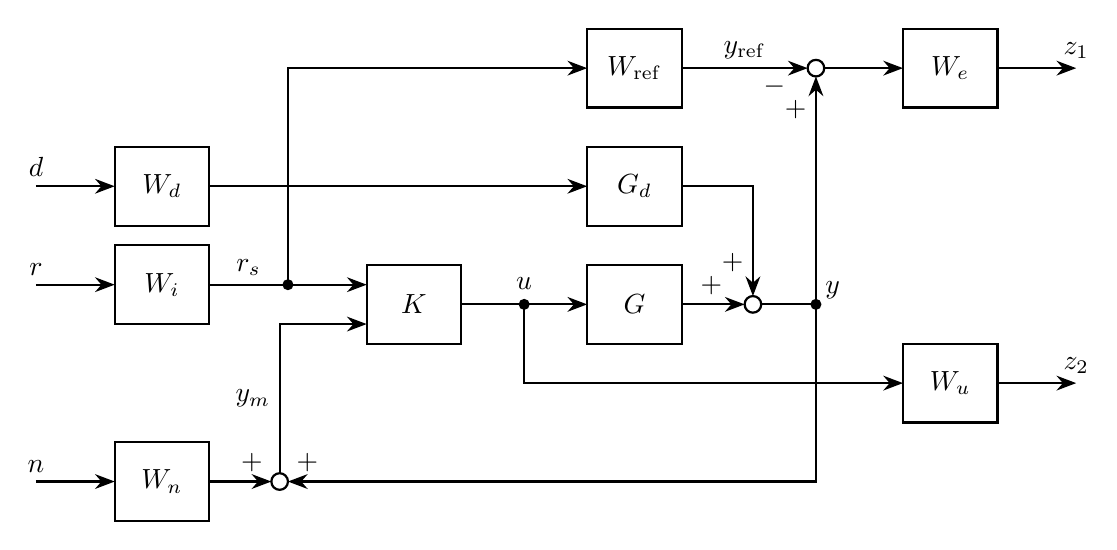
\begin{tikzpicture}
[
% 線と文字の間の間隔を設定
every node/.style={outer sep=0.12cm, inner sep=0},
% 矢印の設定
arrow/.style={-{Stealth[length=0.25cm]}, thick},
% ブロック
block/.style={rectangle, draw, minimum height = 1cm, minimum width=1.2cm,
thick, outer sep = 0},
% 加え合わせ点
sum/.style={thick, circle, draw, inner sep=0, minimum size=6pt, outer sep=0},
% 引き出し点
point/.style={radius=2pt}
]
% ブロックの配置
\node [block] (K) {$K$};
\node [block, right=1.6 of K] (G) {$G$};
\node [sum, right=0.8 of G] (sum1) {};
\node  [block, above = 0.5 of G] (Gd){$G_d$};
\node [block, above = 0.5 of Gd] (Wref) {$W_\mathrm{ref}$};
\node [sum, right=1.6 of Wref](sum2){};
\node [block, right=1 of sum2](We){$W_e$};
\coordinate (K1) at ($(K.north west)!0.25!(K.south west)$);
\coordinate (K2) at ($(K.north west)!0.75!(K.south west)$);
\node [block, left=2 of K1] (Wi) {$W_i$};
\node [block] at (Wi|-Gd) (Wd){$W_d$};
\node [sum, left=1of K2, yshift=-2cm](sum3){};
\node [block] at (Wi|-sum3) (Wn){$W_n$};
\node [block, yshift=-1cm] at (We|-G) (Wu) {$W_u$};

% ブロックの接続
\draw [arrow] (K) -- (G) node [midway, above, yshift=2pt] {$u$};
\fill [point] ($(K.east)!0.5!(G.west)$) circle coordinate (u);
\draw[arrow] (u) |- (Wu);
\draw [arrow] (G) -- (sum1) node[above, xshift=-15pt] {$+$};
\draw [arrow] (Gd) -| (sum1) node [left, yshift=15pt] {$+$};
\draw [arrow] (Wref) -- (sum2) node[below, xshift=-15pt]{$-$} 
node[above, midway]{$y_\mathrm{ref}$};
\draw [arrow] (sum1) -| (sum2) node[left, yshift=-15pt]{$+$};
\draw [arrow] (sum2)--(We);
\draw [arrow] (Wd) -- (Gd);
\draw[arrow] (Wi.east) -- (K1)node[above, pos=0.25]{$r_s$};
\draw[arrow] (sum3) |- (K2);
\path (sum3) -- (sum3|-K2) node [left, midway]{$y_m$};
\draw[arrow] (Wn)--(sum3) node [above, xshift=-10pt]{$+$};
\fill [point] (sum1 -| sum2) circle coordinate (y) node[right, yshift=5pt]{$y$};
\draw [arrow] (y)|-(sum3) node [above, xshift=10pt]{$+$};
\fill [point] ($(Wi.east)!0.5!(K1)$) circle coordinate (rs);
\draw[arrow] (rs) |- (Wref);
\draw[arrow] (We.east) -- +(1cm, 0) node[above]{$z_1$};
\draw[arrow] (Wu.east) -- +(1cm, 0) node[above]{$z_2$};
\draw[arrow] (Wd.west) ++ (-1cm,0) -- (Wd) node[above, pos=0] {$d$};
\draw[arrow] (Wi.west) ++ (-1cm,0) -- (Wi) node[above, pos=0] {$r$};
\draw[arrow] (Wn.west) ++ (-1cm,0) -- (Wn) node[above, pos=0] {$n$};
\end{tikzpicture}
\end{document}